% !TEX root = ../thesis_main.tex
\chapter{Prior Ultrafast Spectroscopy Studies of Carbon Nanotubes}

\section{The Effect of pH on Recombination Dynamics in Single-Walled Carbon Nanotubes}

Based on work in Ref.\ \cite{ostojic2004interband}. Degenerate pump-probe spectroscopy performed using an OPA (See Section \ref{section:opa} for details on OPA function). Pump and probe wavelengths are the same. Optical absorption spectrum in Figure \ref{fig:abs_gordana} shows presence of many different chiralities, including both metallic and semiconducting nanotubes. Dispersion created using HiPCo CNTs dispersed in aqueous solution containing SDS. For pumping and probing within $E_2 H_2$ (defined as $E_{22}$ in Section \ref{section:selection_rules}), only a single exponential decay observed. Interpreted as intra-band relaxation to lower-energy states.
%te
\begin{figure}[ht]
	\centering
	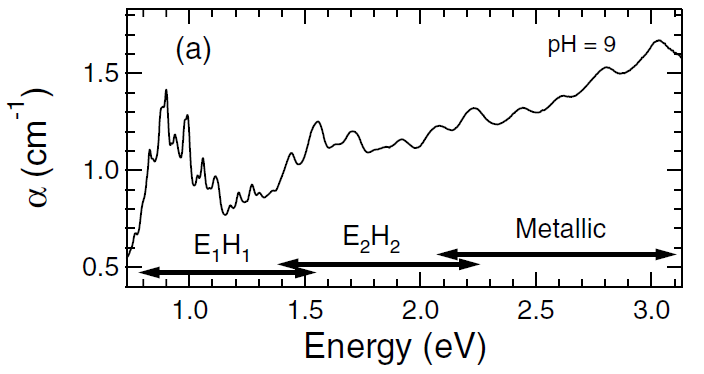
\includegraphics[scale=0.7]{images/chapter_prior_works/abs_gordana}
	\caption{{\color{red} UNFINISHED } Reproduced and modified from Ref.\ \cite{ostojic2004interband}}
	\label{fig:abs_gordana}
\end{figure}

For pumping and probing $E_1 H_1$ (defined as $E_{11}$ in Section \ref{section:selection_rules}), a bi-exponential decay was observed. First exponential process (fast) interpreted as intra-band relaxation. Second exponential decay process (slow) interpreted as inter-band relaxation. Decreasing pH mitigated the presence of a slow exponential decay process as shown in Figure \ref{fig:dtt_ph_gordana}. Interpreted this as a consequence of Burstein-Moss effect. H+ ions of lower pH act dope CNTs, believed that this may cause Fermi level to be somewhere within the conduction band for some population of CNTs such as metallic tubes.

\begin{figure}[h]
	\centering
	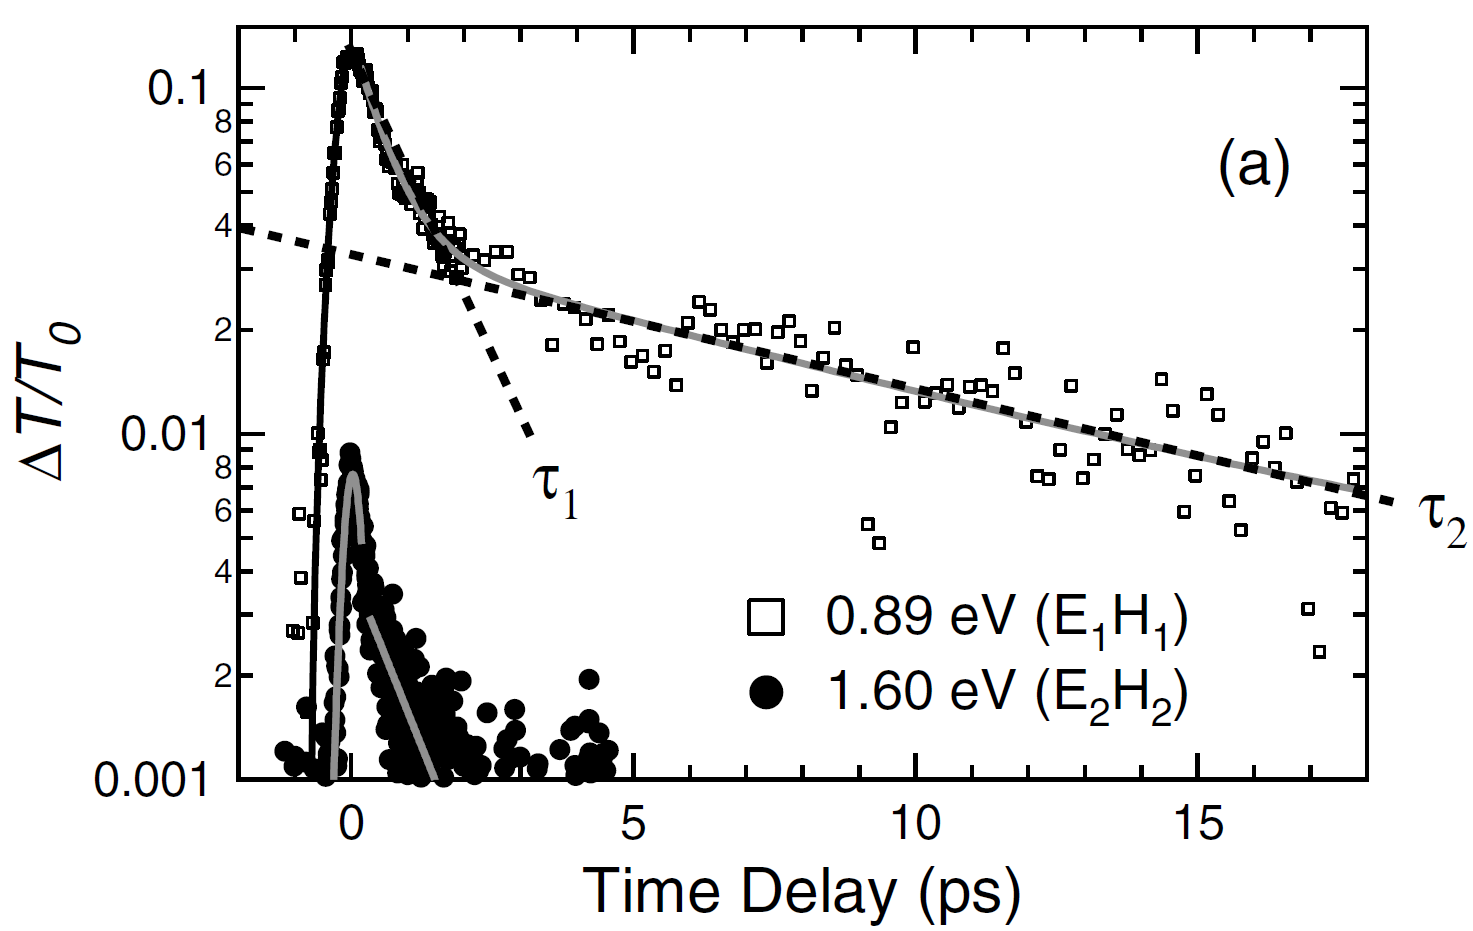
\includegraphics[scale=0.3]{images/chapter_prior_works/dtt_gordana}
	\caption{{\color{red} UNFINISHED } Reproduced and modified from Ref.\ \cite{ostojic2004interband}}
	\label{fig: abs_gordana}
\end{figure}

\begin{figure}[h]
	\centering
	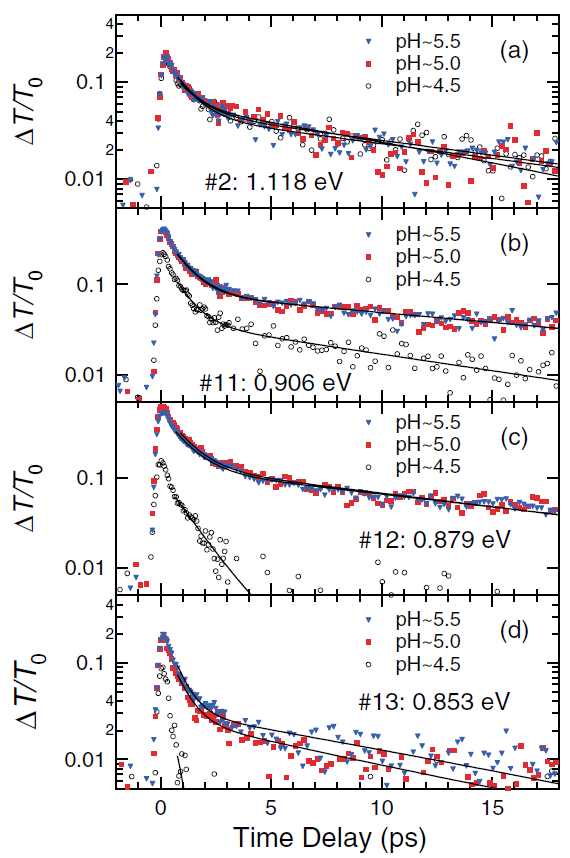
\includegraphics[scale=0.7]{images/chapter_prior_works/dtt_ph_gordana}
	\caption{{\color{red} UNFINISHED } Reproduced and modified from Ref.\ \cite{ostojic2004interband}}
	\label{fig:dtt_ph_gordana}
\end{figure}

Manzoni et.\ al.\ measured intra-band relaxation rates from $E_{22}$ states to $E_{11}$ states. Used HiPCo CNT film samples.  Found that this occurs over a timescale of 150 fs \cite{manzoni2005intersubband}.

Exciton-Exciton annihilation \cite{valkunas2006exciton, yuma2013biexciton}.
They also show that exciton-exciton annihilation occurs over a time scale such that it is hard to reach Mott densitty of excitons where excitons immediately dissociate to form plasma of free carriers. These a
Apparently, excitons dissociate into free electron-hole pairs before recombination occurs \cite{kumamoto2014spontaneous}.
\section{Exciton-Exciton Annihilation}
Efficient exciton-exciton annihilation \cite{murakami2009existence}.

\section{Summary}
